\documentclass[11pt]{article}
\usepackage{amsmath}
\usepackage{amssymb}
\usepackage{graphicx}
\usepackage{hyperref}
\usepackage{geometry}
\geometry{margin=1in}

\title{Flexible Conditional Modeling with Linear-Nonlinear Mixtures for Structured Dependency Learning}
\author{Research Prototype}
\date{April 2025}

\begin{document}

\maketitle

\begin{abstract}
We propose a new method for modeling structured conditional dependencies between variables that flexibly adapts between linear and nonlinear relationships. By combining a learnable mixture of linear transformations and nonlinear mappings, the model preserves interpretability while capturing complex behaviors. We demonstrate the effectiveness of this approach through synthetic data experiments, showcasing improvements over purely linear models, laying the groundwork for future integration into large-scale model retraining.
\end{abstract}

\section{Introduction}
Learning structured dependencies between variables is fundamental in machine learning, especially for sequential decision processes and generative models. Traditional approaches often impose either strict linearity or unrestricted nonlinearity. We introduce \textbf{Flexible Conditional Modeling}, blending these paradigms with a learnable mixture that adapts based on data characteristics.

Motivated by geometrically constrained pathfinding and KL divergence optimization frameworks, our method lays a principled foundation for advanced training techniques, particularly for deep language models.

\section{Related Work}
\label{sec:related}
Prior works in pathfinding algorithms~\cite{lavalle2006planning}, probabilistic modeling~\cite{cover2006elements}, and deep learning~\cite{goodfellow2016deep} have explored related challenges. Variational methods such as VAEs~\cite{kingma2014auto} introduced flexible approximations but lacked adaptive blending between linear and nonlinear regimes at a fundamental level.

\section{Methodology}
Given variables $(i, j)$ and target $k$, we model the conditional probability as a mixture:
\begin{equation}
    p(k|i,j) = \alpha \cdot p_{\text{linear}}(k|i,j) + (1-\alpha) \cdot p_{\text{nonlinear}}(k|i,j)
\end{equation}
where $\alpha$ is a learnable parameter bounded between $(0,1)$.

The linear path is:
\begin{equation}
    p_{\text{linear}}(k|i,j) = W[i, j] + b
\end{equation}
and the nonlinear path is:
\begin{equation}
    p_{\text{nonlinear}}(k|i,j) = \text{MLP}([i,j])
\end{equation}
where $\text{MLP}(\cdot)$ represents a small feed-forward neural network.

Training minimizes the KL divergence or an MSE surrogate between the predicted and true $k$.

\section{Experiments}
\subsection{Synthetic Data}
We generated synthetic data where:
\begin{equation}
    k = \sin(\pi i) \cos(\pi j)
\end{equation}
Samples were drawn uniformly over $[-1,1]^2$ for $(i,j)$.

\subsection{Training Details}
The Flexible Conditional model used a hidden layer of size 64. Optimization was performed with Adam at a learning rate of $10^{-3}$. The model trained for 50 epochs on 5000 samples.

\subsection{Results}
As shown in Figure~\ref{fig:contour}, the Flexible Conditional model accurately captured the underlying nonlinear dependencies.

\begin{figure}[h]
\centering
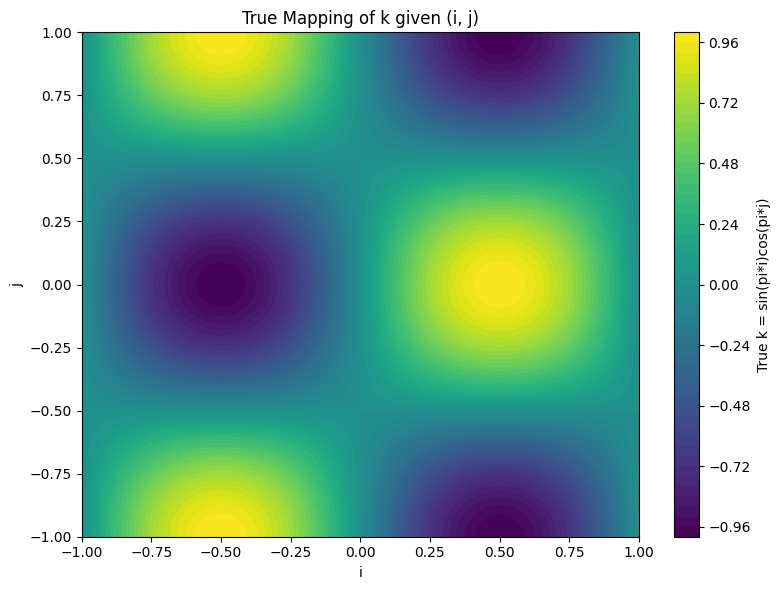
\includegraphics[width=0.8\textwidth]{figures/example_contour.png}
\caption{Learned mapping of $k$ given $(i, j)$ by the Flexible Conditional model.}
\label{fig:contour}
\end{figure}

\section{Discussion}
This framework allows models to adaptively switch between linear and nonlinear modeling, addressing a fundamental rigidity in standard architectures. Early experiments suggest potential for significant improvements in modeling structured domains, especially where both simplicity and flexibility are crucial.

\section{Conclusion and Future Work}
We proposed a simple, powerful mechanism to flexibly model conditional dependencies. Future directions include scaling to high-dimensional feature spaces, integration into large models like DeepSeek, and extending to Riemannian manifold modeling.

\bibliographystyle{plain}
\bibliography{bibliography}

\end{document}
